\documentclass[11pt,a4paper]{article}
\usepackage[T1]{fontenc}
\usepackage[utf8]{inputenc}
\usepackage{amsmath,amsthm,mathtools}
\usepackage{newpxtext,newpxmath}
\usepackage[margin=25mm,headheight=16pt]{geometry}
\usepackage{microtype}
\usepackage{booktabs,tabularx,longtable,array}
\usepackage{enumitem}
\usepackage{listings}
\usepackage{xcolor}
\usepackage[most]{tcolorbox}
\usepackage{tikz}
\usetikzlibrary{arrows.meta,positioning,calc}
\usepackage{fancyhdr}
\usepackage{hyperref}
\usepackage{bookmark}
\definecolor{ink}{HTML}{203E35}
\definecolor{soft}{HTML}{F0F5F2}
\definecolor{muted}{HTML}{54655E}
\hypersetup{colorlinks=true,linkcolor=ink,citecolor=ink,urlcolor=ink,
 pdftitle={Fennel: A Proof Language of Stable Objects and Explicit Requirements},
 pdfauthor={OpenAI},pdfsubject={Fourth-round proof-language proposal}}
\urlstyle{same}
\pagestyle{fancy}
\fancyhf{}
\fancyhead[L]{\small\textsc{Fennel}}
\fancyhead[R]{\small Stable objects, explicit requirements}
\fancyfoot[C]{\thepage}
\renewcommand{\headrulewidth}{0.3pt}
\setlength{\parindent}{0pt}
\setlength{\parskip}{0.55em}
\setlength{\emergencystretch}{2em}
\setcounter{tocdepth}{1}
\setlist{nosep,leftmargin=1.5em}
\newcolumntype{Y}{>{\raggedright\arraybackslash}X}
\newcolumntype{L}[1]{>{\raggedright\arraybackslash}p{#1}}
\lstdefinestyle{fennel}{basicstyle=\ttfamily\small,columns=fullflexible,
 keepspaces=true,breaklines=true,breakatwhitespace=false,
 frame=single,rulecolor=\color{muted!35},backgroundcolor=\color{soft},
 xleftmargin=0.7em,xrightmargin=0.7em,framexleftmargin=0.4em,
 showstringspaces=false,tabsize=2,aboveskip=0.9em,belowskip=0.7em}
\lstset{style=fennel}
\newtcolorbox{principle}[1][]{colback=soft,colframe=ink!55,boxrule=.5pt,
 arc=0pt,left=9pt,right=9pt,top=7pt,bottom=7pt,#1}
\newtheorem{theorem}{Theorem}[section]
\newtheorem{proposition}[theorem]{Proposition}
\newtheorem{lemma}[theorem]{Lemma}
\theoremstyle{definition}
\newtheorem{definition}[theorem]{Definition}
\theoremstyle{remark}
\newtheorem{remark}[theorem]{Remark}
\newcommand{\code}[1]{\texttt{\detokenize{#1}}}
\newcommand{\Prop}{\mathsf{Prop}}
\newcommand{\Spec}{\mathsf{Spec}}
\newcommand{\Beh}{\mathsf{Beh}}
\newcommand{\Req}{\mathsf{Req}}
\newcommand{\Cl}{\mathsf{Cl}}
\newcommand{\Min}{\mathsf{Min}}
\newcommand{\NN}{\mathbb N}
\newcommand{\ZZ}{\mathbb Z}
\newcommand{\QQ}{\mathbb Q}
\newcommand{\RR}{\mathbb R}
\newcommand{\sem}[1]{\llbracket #1\rrbracket}
\newcommand{\fname}{\textsc{Fennel}}

\begin{document}
\begin{titlepage}
\vspace*{10mm}
{\color{muted}\large FOURTH-ROUND PROPOSAL\par}
\vspace{8mm}
{\color{ink}\fontsize{44}{48}\selectfont Fennel\par}
\vspace{6mm}
{\LARGE A Proof Language of Stable Objects\par and Explicit Requirements\par}
\vspace{7mm}
{\large Behavioral types, proof-carrying frontiers,\par and a finite authoring prototype\par}
\vspace{11mm}
\begin{principle}
\large A mathematician should state the argument, not the plumbing.\par
\normalsize The omitted work must nevertheless have a precise target,\newline
an explicit context, and a checkable route back to the statement.
\end{principle}
\vspace{8mm}
\textbf{Central proposal.} Extend Lean's \emph{elaborated typing discipline} with
property-implicit arguments, relational behavioral contracts, and a
proof-carrying description of what remains to be proved. Keep ordinary Lean
terms as the verification boundary. Treat alternative sufficient premises as
first-class mathematical information rather than as an unexplained tactic failure.

\textbf{Concrete contribution.} This package includes an executed finite-Horn
parser and planner, an independent certificate checker for that fragment, and
an exporter of ordinary conditional Lean theorems. It does not include a
working dependent Lean elaborator or a new kernel.
\vfill
{\large 6 September 2026\par}
\vspace{2mm}
{\color{muted}Prepared for Vladimir Reshetnikov's proof-language brainstorm campaign\par}
\end{titlepage}

\begin{abstract}
The third-round proposals have already converged on a sensible foundation:
keep mathematical objects fixed while their proved properties accumulate;
separate chosen structures from propositions; and check all generated work in
Lean. A fourth proposal should not rename this consensus. Fennel instead makes
one unfinished part precise: the \emph{residual requirements} of a mathematical
step. Its automatic core propagates finite, proof-carrying antichains of
sufficient assumption sets through a grounded theorem graph. This supplies
alternative routes, operation-specific prerequisites, restricted-method proofs,
and honest failure states. The algorithm has a precise relative-completeness
result, a visible exponential worst case, and an executable reference model.

Around this core, Fennel supplies a small mathematical surface, property-implicit
binders, dependent behavioral contracts, typed locality and approximation
relations, and explicit construction boundaries. Worked studies use the actual
q-Pochhammer and autonomous-derivative proofs in ProveIt, the Frey model transport
and tensor-representability proofs in the Fermat repository, and Leant's
candidate-provenance interfaces. A certificate-oriented CAS boundary and a
realization-aware synthesis boundary complete the architecture. We distinguish
written metatheory, executed finite tests, historical checks reported by the
previous syntheses, and work not yet implemented. The proposal's success
criterion is better authoring and repair than equally equipped Lean, not a
smaller screenshot or a more impressive vocabulary.
\end{abstract}

\tableofcontents
\clearpage

\section{What the fourth round should add}
\label{sec:position}

\subsection{The question is no longer whether to use refinements}
The two requested reports, \emph{From Properties to Proof Obligations} and
\emph{Nine Refinements}, have been read at the same immutable Brainstorm
snapshot. Their reconciled conclusions are unusually clear: the nine designs
largely share one calculus, some small semantic components have been checked,
but the authoring interface and its benefit have not been demonstrated
\cite{synA,synB}. Fennel adopts that assessment rather than treating agreement
among related proposals as independent experimental evidence.

The most useful next question is not ``what other properties can a type carry?''
Lean can already state arbitrarily complicated predicates. It is this:
\begin{quote}
When a mathematician writes a valid high-level step, can the system expose
exactly the \emph{available sufficient ways} to justify it, without altering
its meaning or asking the author to reconstruct the library's calling convention?
\end{quote}

A type such as ``continuous function'' helps only if the elaborator can retain
which function and topology it describes, apply the right theorem, derive the
other premises, and explain any remainder. A record with many Boolean-looking
labels does not solve those problems. Neither does an unconstrained language
model that produces a plausible proof of a nearby proposition.

\subsection{The inherited foundation and Fennel's increment}
\begin{center}\small
\begin{tabularx}{\textwidth}{@{}L{.27\textwidth}YY@{}}
\toprule
Concern & Inherited from round three & Fennel's proposed increment\\
\midrule
Properties & Evidence attached to a fixed term. & Property-implicit consumers return a typed residual requirement, not an unexplained failure.\\
Inference & Bounded demand search and finite qualifier closure. & An executable antichain algorithm for alternative sufficient supports, with proof certificates and explicit limits.\\
Meaning & Structures and statement parameters are fixed before search. & A staged elaboration protocol with separate authority for proof holes and specified construction holes.\\
Methods & A required reason differs from a hint. & Restrict the inference graph before constructing a derivation; retain the selected route.\\
Repair & Context-sensitive evidence and explicit transport. & Separate assumption-availability edits from rule, structure, and dependent-context edits.\\
Validation & Compare against equally equipped Lean. & A shipped narrow parser/planner/checker and a falsifiable next-stage evaluation protocol.\\
\bottomrule
\end{tabularx}
\end{center}

The provenance algorithm itself is not historically new. Minimal supporting
environments are central to assumption-based truth maintenance; de Kleer's
account also stresses that a correct maintenance component does not make its
whole surrounding system correct \cite{atms}. The research proposal is the
integration of such proof-carrying supports with fixed Lean statements,
property-aware mathematical elaboration, and a disciplined publication interface.
This attribution matters: a useful fourth iteration should reuse mature ideas,
not claim to have invented them.

\subsection{What was actually inspected}
The source review is deliberately bounded. It includes the two main synthesis
sources, Trellis's core and finite-qualifier sections, two complete ProveIt
calculus files, two complete Fermat solution files, and selected Leant source
ranges \cite{synA,synB,trellis,qpoch,ode,frey,tensor,leantV,leantH}.
It is not a review of every theorem in either mathematical repository. The
external source pins and reviewed paths are recorded in
\code{evidence/source_manifest.json}.

The reconciled reports supply several important corrections. Moraine's
finite-tensor exposition omitted the factors' finite/free assumptions; the
original Lean theorem includes them. Unrestricted affine-coefficient equality
is not complete for source behavior on \code{List Empty}. A successful checker
needs soundness, not completeness, to justify a positive answer. These are
not incidental editorial matters: each is a regression case for the proposed
language \cite{synA,synB}.

\section{A diagnosis from the actual Lean examples}
\label{sec:diagnosis}

\subsection{There are several different kinds of verbosity}
The files illustrate at least four costs that must not be conflated.
\emph{Mathematical detail} includes the premises that make a cancellation,
interchange, or induction valid. \emph{Interface detail} includes argument order,
coercions, projections, and which extensionality lemma to use.
\emph{Representation detail} includes proving that integer and rational
expressions denote the same intended coefficient. \emph{Environment detail}
includes imports, instance selection, and generated configuration. A new surface
may hide the last three, but it must not silently discard the first.

The q-Pochhammer derivative file is a good example. The general finite-product
rule is mathematically straightforward. Its formal proof explicitly assembles
the derivative of each factor, invokes the finite-product theorem, and aligns
scalar multiplication, signs, and multiplication order. Its second theorem
requires nonzero factors to obtain a quotient-shaped expression
\cite{qpoch}. The first group of details is promising automation work. The
nonzero assumptions in the second theorem are not merely inconvenient syntax.

The autonomous-derivative theorem is already a well-factored abstraction. Its
induction step turns equality throughout an open region into equality near the
current point before differentiating \cite{ode}. The language should make that
step natural while preserving its quantifier scope. Calling the existing proof
``badly verbose'' would miss that it already isolates the mathematical mechanism.

\subsection{Bundling alone is not the answer}
The Fermat development already uses a \code{FreyPackage}. Its integral-to-rational
curve theorem nevertheless needs precise divisibility and cast arguments
\cite{frey}. Thus the missing feature is not simply ``put more hypotheses in a
structure.'' A consumer needs the relevant consequences of a bundle, at the
right operation, with the right support.

The tensor-representability file similarly constructs a witness, its ring and
algebra structures, finite/free properties, a family of equivalences, and its
naturality law \cite{tensor}. Those components cannot be compressed into a
single unexplained ``finite algebra'' annotation. They are different kinds of
data and evidence. The implementation must know which ones may be inferred,
which ones must be constructed, and which relations bind the configuration.

\subsection{The working hypothesis}
Fennel's hypothesis is that a small number of \emph{consumer-oriented interfaces}
can eliminate repeated interface work while keeping the mathematical argument
visible. The author should normally say ``differentiate on this open region,''
``transport this exact quotient,'' or ``compose these lawful maps.'' The system
should supply theorem applications and proof plumbing. When it cannot, the
answer should be a useful mathematical requirement, not just the internal
metavariable at which elaboration stopped.

This is a hypothesis about an interface, not evidence of a productivity gain.
Every inspected file in this article is development material. None will be
called a held-out test.

\section{The surface: state the argument, retain its commitments}
\label{sec:surface}

\subsection{Three verbs with different authority}
Fennel distinguishes \code{fix}, \code{derive}, and \code{construct}.
\code{fix} introduces or selects data whose meaning is thereafter stable.
\code{derive} requests evidence about those data.
\code{construct} authorizes a new witness satisfying a fixed specification.
The following is \emph{proposed full-language syntax}, not accepted Lean or
syntax supported by the finite prototype:
\begin{lstlisting}
context real_analysis
fix U : Set Real with open U
fix W, phi : Real -> Real
assume flow : forall x in U, derivative W at x is phi(W(x))

construct G : Nat -> Real -> Real satisfying recurrence
  using polynomial_recurrence

derive forall n, on U, derivative[n] W = G(n) after W
  by induction n keeping the point general

audit statement, remaining_requirements, required_methods
\end{lstlisting}

The phrase \code{keeping the point general} is not decorative prose. It
selects an induction schema whose hypothesis retains the universal point
binder. Conversely, \code{using polynomial_recurrence} does not let the system
change the recurrence or select a different function under the same printed
name. The requested witness and its specification are explicit construction
inputs.

\subsection{Mathematical syntax is controlled, not unrestricted English}
The proposed surface has ordinary binders, formulas, calculation blocks,
induction, cases, constructions, and theorem-backed method applications. Natural
language surrounds these forms as commentary; it does not secretly change the
logical grammar. Existing Lean terms remain an escape hatch for definitions,
proofs, and unusual dependent constructions.

Each mathematical command has two independently useful views. The compact
view shows the statement, domain, quantifiers, result kind, and named reason.
The expanded view shows the instantiated theorem, inserted evidence,
remaining premises, and resulting Lean term. A reader should not need to expand
routine arithmetic, but should never have to expand the proof to discover that
an equality was only almost everywhere or conditional on a denominator.

\subsection{A small example of honest compression}
\begin{lstlisting}
fix a, q : K and n : Nat
let P(x) := product j < n of (1 - x*q^j)

derive derivative P at a
  = - sum j < n of q^j * product i < n, i != j of (1-a*q^i)
  via finite_product_rule

request the logarithmic form
  = -P(a) * sum j < n of q^j/(1-a*q^j)
\end{lstlisting}
The second request may expose a frontier
\[
 \forall j<n,\quad 1-aq^j\ne0.
\]
If that condition has not been proved, the compact view says so. It may also
show the unconditional product-form theorem already obtained. It may not
publish the requested quotient form merely because the product form is true.
The result's chosen representation can affect its mathematical validity.

\section{Extending the type system without confusing its layers}
\label{sec:types}

\subsection{What Lean already provides}
Lean's dependent types, inductive types, propositions, and proof terms are
sufficient to encode the proposed properties and contracts. Its elaborator
produces terms that a small kernel checks \cite{leanTypes}. Thus ``extend the
type system'' has two quite different meanings: extend what authors can write
and infer, or extend the kernel's primitive typing and conversion rules.
Fennel initially chooses the former, while specifying a measured research
path for the latter in Section~\ref{sec:kernel}.

\subsection{Fixed data and proof-only overlays}
Let $\Sigma$ be the selected structure environment and $\Gamma$ an ordered Lean
context. A property-aware judgment has the form
\[
 \Sigma;\Gamma\vdash e:A\;\mathsf{with}\;\rho,
 \qquad \rho=\{P_1(e),\ldots,P_k(e)\}.
\]
The denotation is the same term $e:A$ and proofs $p_i:P_i(e)$. It does not
replace $e$ by a succession of newly packaged subtype values.

At an exported interface, packaging is appropriate:
\[
 \operatorname{Ref}(A,P):=\{x:A\mid P(x)\}.
\]
Locally, a binder such as ``$x:\RR$ with $0<x$'' instead elaborates to
$(x:\RR)(h:0<x)$. Both representations are useful; neither should be forced
at every use. The preceding proposals make this same distinction
\cite{synA,synB,trellis}.

\subsection{Property-implicit arguments}
Fennel adds a dedicated binder category:
\begin{lstlisting}
context field K
method cancel_left(x, y, z : K)
  requires x != 0
  accepts x*y = x*z
  ensures y = z
\end{lstlisting}
A \code{requires} argument is a proof parameter whose target is resolved by
the property engine. It is not a new logical assumption, a global typeclass
instance, or a runtime test. A registered method is backed by an ordinary Lean
theorem or a checked wrapper with this interface.

This category is useful because a mathematical property has different inference
behavior from a structure dictionary. Choosing a multiplication or topology
changes meaning. Producing another proof of a fixed nonzero proposition does
not. The engine may use a local \code{Fact} bridge where a legacy API expects an
instance, but it should not turn every derived fact into globally competing
instance search \cite{synA,synB}.

\subsection{Refinement consequence and equality transport}
There are only a few logical rules:
\[
 \frac{p:P(e)\qquad h:\forall x,\ P(x)\to Q(x)}{h\,e\,p:Q(e)},
 \qquad
 \frac{p:P(e)\qquad q:Q(e)}{\langle p,q\rangle:P(e)\land Q(e)}.
\]
If $h:e=e'$, equality elimination transports $P(e)$ to $P(e')$.
If the bridge is merely $P(e)\leftrightarrow Q(e')$, its appropriate implication
transports the proposition, without asserting equality of objects.
An isomorphism, a homomorphism, and an approximate observation each require
consumer-specific theorems.

The choice of structures is part of the elaborated proposition. Two terms
printed as $x+y$ need not have the same meaning under different addition
structures. A proof cache therefore indexes the actual expression and context,
not its typography. Proof irrelevance does not identify different structures.

\subsection{Incomplete typing has an explicit residual}
For incomplete authoring we write
\[
 \Sigma;\Gamma\vdash e\Leftarrow A\;\mathsf{with}\;\rho
 \quad\dashv\quad\Delta.
\]
Here $\Delta$ is an ordered telescope of still-open obligations. The resulting
proof expression is well typed only in the extended context or in a Lean
metavariable state representing those obligations. It is not a proof in
$\Gamma$ until the obligations are discharged. An explicit conditional theorem
may abstract them; a completed theorem may not acquire extra assumptions
silently.

There are three statuses: a completed proof; a conditional route with stated
remaining obligations; and an unsuccessful or incomplete search. This is a
static logical distinction, not merely different colors in the editor.

\section{Behavioral types: properties of computations and configurations}
\label{sec:behavior}

\subsection{The total-function contract}
For $f:A\to B$, $P:A\to\Prop$, and $Q:A\to B\to\Prop$, define
\[
 \Beh(f;P,Q):=\forall x:A,\ P(x)\to Q(x,f(x)).
\]
This says what a \emph{fixed total function} guarantees on admissible inputs.
It differs from a function $\{x:A\mid P(x)\}\to B$ and from a partial
computation returning an option. Fennel preserves the semantics of imported
Lean definitions; it does not reinterpret totalized division or differentiation
as partial functions without an explicit interface.

An executable synthesis request may instead ask for
\[
 \{f:A\to B\mid\Beh(f;P,Q)\}.
\]
Here the function is authorized construction data. The specification is fixed.
A proof that a witness exists in $\Prop$ is not automatically executable data;
a constructive implementation or an explicitly declared noncomputable choice
is a separate decision.

\subsection{Consequence and composition with the actual intermediate}
If $\Beh(f;P,Q)$, $P'(x)\to P(x)$, and $Q(x,y)\to Q'(x,y)$, then
$\Beh(f;P',Q')$. A stronger input restriction and a weaker promised result are
safe. This does not mean that a replacement implementation may demand a
stronger precondition from its existing clients.

Suppose
\[
 \Beh(f;P,Q),\qquad \Beh(g;R,S),\qquad
 \forall x,y,\ P(x)\to Q(x,y)\to R(y).
\]
Then the composite has the dependent guarantee
\begin{equation}\label{eq:comp}
 \forall x,\ P(x)\to
 Q(x,f(x))\land S(f(x),g(f(x))).
\end{equation}
The proof applies the first contract at $x$, proves the second precondition
at $f(x)$, and applies the second contract there. The intermediate is not an
arbitrary existential witness that can be replaced by a more convenient value.
This is the compositional contract inherited from round three
\cite{synA,synB}.

For a postcondition $T(x,g(f(x)))$, a final implication from the conjunction in
\eqref{eq:comp} is required. Fennel can derive this bridge or request it. A
matching arrow type $A\to B\to C$ alone is not the bridge.

\subsection{Relational behavior is not a collection of unary tags}
Monotonicity compares two evaluations. A Lipschitz bound compares distances.
Naturality compares two paths through a diagram. Inverse-pair behavior relates
two functions. The basic representation must therefore permit predicates on
whole configurations:
\[
 \mathcal R(f,g,\mu,\alpha,\ldots):\Prop,
\]
not only predicates on the output of one call.

For sorting, length preservation is too weak. Sortedness alone admits an empty
result. The usual contract requires both an order condition and permutation of
the \emph{actual input}; stability, when requested, adds another relation.
Fennel never treats these as successively higher points on one universal
``strength scale.'' Their implications depend on the domain and definitions.

\subsection{Effects and proof requirements are separate axes}
Logical facts are reusable: a nonzero proof may be used twice. They are not
linear resources that disappear after consumption. Approximation precision may
change under an operation, but that is a theorem about a relation, not the
consumption of a proof token. Runtime state, exceptions, and nondeterminism
belong to an effect specification. Lean's monadic verification-condition
machinery and the Dijkstra-monad tradition are relevant existing mechanisms,
not inventions of Fennel \cite{mvcgen,dm}.

A service timeout belongs to neither a mathematical precondition nor a theorem's
conclusion. It means that a search did not finish under the allocated budget.

\section{Proof-carrying frontiers}
\label{sec:frontiers}

\subsection{Why a set of missing goals is not enough}
Suppose a requested property can be proved either from $A$ and $B$, or from $C$.
Showing all three as mandatory missing premises is misleading. Showing only
one route may conceal a much easier argument. Fennel retains the alternatives
\[
 \{\{A,B\},\{C\}\},
\]
each with its own derivation. The interface may initially display one route
for readability, but must disclose alternatives and whether the search was
complete in its declared fragment.

These are \emph{sufficient registered supports}, not the logically weakest
preconditions of the theorem. A different library lemma may prove the target
from $D$, and a semantically weaker proposition may be absent from the
vocabulary altogether. The mathematical distinction is made precise below.

\subsection{The finite ground instance}
\begin{definition}[Frontier instance]
Fix a finite set $V$ of well-typed propositions in a fixed context; a finite
set $H$ of named, independent proof-assumption roots; a set $B\subseteq V$ of
currently available base facts; and a finite set $\mathcal R$ of theorem-backed
rules
\[
 p_1,\ldots,p_k\Longrightarrow q,\qquad p_i,q\in V.
\]
Every root $h\in H$ names a proposition $\alpha(h)\in V$. Every rule has an
ordered premise list and an accepted term of that implication type. Empty
premise lists are permitted only with their supplied proof.
\end{definition}

``Ground'' means that data, structures, and universe choices are fixed in the
local context. It does not mean numerical. The proposition $0<x$ is ground
after an arbitrary real $x$ has been fixed. Universal reasoning occurs when
that local proof is later abstracted, not by enumerating real inputs.

For $S\subseteq H$, let
\[
 \Cl(S)=\text{the least rule-closed set containing }
 B\cup\{\alpha(h):h\in S\}.
\]
A support label for $q$ is an antichain $L(q)\subseteq\mathcal P(H)$: no member
properly contains another. Its intended denotation is the upward-closed set
\[
 \uparrow L(q)=\{S\subseteq H:\exists T\in L(q),\ T\subseteq S\}.
\]
Fennel retains a proof derivation for every stored minimal support.

\subsection{The algorithm}
Initialize $L(q)$ with $\{\varnothing\}$ for a base fact and with $\{\{h\}\}$
for each root naming $q$; minimize under inclusion. For each rule, combine one
support for each premise and insert their union at the conclusion:
\begin{equation}\label{eq:frontier-update}
 L(q)\gets\Min\left(L(q)\cup
 \left\{S_1\cup\cdots\cup S_k:S_i\in L(p_i)\right\}\right).
\end{equation}
Retain the rule instance and references to the selected premise derivations.
Continue fairly until no label changes. With no premises, the product has one
empty tuple and its support union is empty. An unseeded cycle produces nothing.

\begin{lstlisting}
for each initially available proof:
  insert its empty support and derivation
for each pending proof root h:
  insert support {h} and the root derivation
repeat until stable:
  for each permitted ground rule r:
    for each tuple of currently retained premise routes:
      S := union of their supports
      if no existing support for the conclusion is a subset of S:
        remove supports strictly containing S
        retain S and the application of r to those routes
\end{lstlisting}

The implementation in this package uses this simple algorithm rather than an
optimized solver. It deliberately makes the state and certificate format easy
to inspect.

\subsection{A precise theorem, including its limits}
\begin{theorem}[Finite frontier theorem]\label{thm:frontier}
For a fixed finite frontier instance, exhaustive fair propagation terminates.
Its final labels satisfy
\begin{equation}\label{eq:exact-closure}
 q\in\Cl(S)\quad\Longleftrightarrow\quad
 \exists T\in L(q),\ T\subseteq S
 \qquad(S\subseteq H).
\end{equation}
Every retained route yields a proof of $q$ from the base proofs, its named
assumptions, and the registered rule proofs. The final antichains are unique,
although selected derivations need not be. No consistency assumption on the
mathematical context is needed for soundness.
\end{theorem}
\begin{proof}
Interpret each label by its upward closure. An insertion never removes an
upward-closed possibility: discarding a support containing a newly inserted
smaller one preserves coverage. Every successful insertion adds at least one
previously uncovered pair $(q,S)$, namely its own conclusion and support.
There are at most $|V|2^{|H|}$ such pairs, so there can be only finitely many
successful insertions.

For soundness, a base derivation uses its supplied proof, a root derivation its
assumption, and a rule derivation applies its supplied implication to previously
constructed premise derivations. The union of supports contains every needed
assumption. The proof graph points to earlier nodes and is acyclic even when
the rule graph is cyclic. Weakening supplies the proof under any larger $S$.

For completeness relative to $\Cl$, induct on a finite forward derivation of
$q\in\Cl(S)$. A base fact has empty support, and an enabled root has a singleton
support contained in $S$, or a smaller support replacing it. At a rule step,
the induction hypotheses give premise supports contained in $S$. At a fixed
point their union is covered by a conclusion support. Thus the right-hand side
of \eqref{eq:exact-closure} holds. The converse is soundness. Every upward-closed
set has a unique inclusion-minimal antichain, proving the claimed uniqueness.
\end{proof}

This theorem is not completeness for Lean, for all mathematical implications,
or for theorem instantiation. It also does not say that a root in a minimal
support is mathematically indispensable. It says that no proper subset of that
support derives the target in this fixed forward-rule system with these base
facts. Different proofs of a rule may themselves have different dependencies
outside the root vocabulary.

\subsection{Residual formulas and new evidence}
When $K\subseteq H$ has been discharged, the remaining support family is
\[
 \Min\{S\setminus K:S\in L(q)\}.
\]
Its associated sufficient condition is
\begin{equation}\label{eq:residual}
 R_q=\bigvee_{S\in L(q)}\ \bigwedge_{h\in S\setminus K}\alpha(h).
\end{equation}
By substituting the known root proofs into each retained derivation, then using
disjunction elimination, one obtains $R_q\to q$. An empty conjunction is true;
an empty disjunction is false, so the latter implication gives no evidence for
$q$ and does not prove $\neg q$.

A single printed ``missing $P$'' message should therefore mean ``$P$ is required
by this displayed sufficient route,'' not ``$P$ is necessary for the theorem.''
A proof of a conditional route is not permission to append its condition to the
author's sealed theorem statement.

\subsection{The unavoidable exponential case}
For each $i=1,\ldots,k$, let either root $a_i$ or root $b_i$ prove $p_i$, and
let all $p_i$ together prove $q$. The minimal supports for $q$ choose one root
from each pair. There are $2^k$ incomparable choices. Therefore even the output
may be exponential; the linear bookkeeping bound for ordinary finite closure
does not apply to enumerating every frontier.

Fennel should provide a fast first-route mode and a separately bounded
alternative-route mode. The prototype instead exposes node and rule-combination
budgets directly. If a budget expires, every emitted route still has a checked
certificate, but the completeness flag is false. Dropping alternatives must
never be disguised as proving that no alternative exists. Decision diagrams or
symbolic provenance could compress some workloads later; they do not remove
the worst-case problem or eliminate the need for proof reconstruction.

\subsection{What this is not: default reasoning}
Although the data structure is related to an ATMS, an \code{ask} root is not a
belief adopted by default. It is an outstanding proof parameter. Fennel does
not exclude inconsistent assumption sets merely because they are inconvenient:
proof by contradiction is legitimate mathematics. Contradictions become
ordinary evidence, with their support, and a requested method may restrict
whether an explosion route is allowed. There is no negation-as-failure rule.

\section{From Lean theorems to a finite inference problem}
\label{sec:grounding}

\subsection{Registration describes an existing theorem}
A method registration names a Lean declaration, identifies its data and
structure parameters, distinguishes proof premises, and identifies the
conclusion. The registration does not define the theorem's meaning. The
elaborator must inspect the actual declaration type and reject mismatched
metadata. Project-owned wrappers are preferable when a library theorem's
interface is too dependent or too general for a stable user-facing method.

For example, an exact-rational-quotient wrapper may expose an integer numerator,
an integer denominator, divisibility, and denominator nonzeroness. The source
Frey proof uses the available rational cast theorem; Fennel need not assume
that every version of a similarly named generic cast lemma has the same
argument order \cite{frey}. The wrapper and toolchain pin are the contract.

\subsection{A bounded grounding policy}
The full proposed engine uses a \emph{fixed-term pool}. Initially this contains
the elaborated target's subterms, explicitly selected local objects, and the
arguments of registered local facts. Structures and universe instantiations
are retained. For each selected consumer, the engine matches its conclusion
against the demanded proposition and instantiates only its data parameters.
Every resulting premise becomes a candidate demand.

A registration may include a finite term-producing template, such as the
intermediate $f(x)$ of a contract application. Such templates run only up to a
specified expansion depth and total-node budget. The engine then freezes the
generated proposition and rule set before claiming exhaustive closure. A
result records the expansion bounds, attempted registrations, and rejected or
unsupported instantiations. The finite theorem in Section~\ref{sec:frontiers}
applies to that frozen graph, not to all instances of the underlying theorems.

Rule generation is a separate stage for an important reason. The single schema
$P(x)\to P(f(x))$ can create infinitely many distinct terms. A finite closure
algorithm does not make unconstrained term generation finite. Likewise,
higher-order unification and dependent transport are not free operations merely
because the resulting graph is small.

\subsection{Use existing automation rather than duplicating it}
An unresolved leaf may be delegated to a named service: direct theorem lookup,
Lean tactics, \code{fun_prop} in its supported property classes, arithmetic
normalization, a proof-producing solver, or Leant synthesis
\cite{funprop,leanTactics,leantV}. On success, the leaf receives the returned
proof of the exact fixed proposition. It can then become a base fact in a
subsequent frontier phase. A solver failure does not create a negative fact.

This two-stage arrangement is deliberately modest. The finite engine is not
intended to rediscover every continuity theorem or replace Lean's existing
unification. Its value would be the control and explanation of how existing
services compose. That incremental value must be measured against the same
services available without Fennel.

\subsection{Dependent obligations are not just sets of atoms}
Suppose a method first constructs $n:\NN$ and then needs a vector of length $n$.
The obligations form a telescope, not two independent propositions. A pending
witness cannot be flattened into an untyped atom called ``vector exists.''
Fennel creates an explicit construction stage, fixes the chosen witness, and
then grounds the subsequent proof requirements in the extended context.

Similarly, a root whose type depends on a previous proof parameter must retain
that dependency, or be represented by a self-contained implication proposition.
The finite prototype assumes independent proposition roots in one fixed
context. Its antichain theorem should not be advertised as a theorem about
arbitrary dependent-context pruning. The full system either closes supports
under telescope dependencies or declines to minimize across such a boundary.

\section{Statement identity, rewriting, and incremental repair}
\label{sec:identity}

\subsection{A sealed request is an elaborated object, not a sentence}
A request consists of the actual target expression, its ordered local context,
selected structures and universes, imported environment identity, authorized
construction mode, and any method or axiom policy. Pretty-printed text is a
view of this request. A digest is a useful integrity check, but it is not a
proof that two meanings coincide.

For the first Lean implementation, use a particularly simple rule: the target
itself contains no unresolved metavariables when sealed. This does not require
solving the new proof goal. The target can contain arbitrary local variables;
the pending proof is a separate metavariable of that fixed type. A construction
request likewise has a fixed type such as $\{x:A\mid\Spec(x)\}$, while the
witness inhabiting it remains to be found. This avoids trying to infer which
unresolved target holes happen to be semantically harmless.

\subsection{The elaboration transaction}
The proposed transaction has four stages.
First, ordinary elaboration fixes the statement and structures, and produces a
reviewable mathematical rendering. Second, property inference and providers
work against a copy of that context with the target frozen. Third, a returned
candidate is rechecked in the original context against the original target;
no unapproved metavariable assignment, local declaration, or imported axiom is
accepted. Finally, the proof and its source correspondence are committed
together. A failed transaction leaves the authored statement unchanged.

\begin{proposition}[Statement noninterference of the specified protocol]
Assume every search transition preserves the sealed target and context, and
acceptance checks the returned term against that target in that context. Then
search cannot change the proposition of an accepted request. Construction may
change its result witness only within the fixed construction specification.
\end{proposition}
\begin{proof}
The sealed request is an invariant of the transition relation. Induction on
any finite sequence of search transitions preserves it. Acceptance therefore
uses the initial target. For a construction request the initial target already
quantifies or packages the authorized witness, so the chosen witness changes
the returned inhabitant, not the type being inhabited.
\end{proof}

This is a specification theorem, not a mechanized proof about a Lean plugin.
An implementation that permits a unification side effect to modify a protected
metavariable violates its premise. Tests must exercise the actual MetaM and
elaboration boundaries rather than only compare saved strings. The proposed
protocol is intentionally stronger and easier to audit than a heuristic
classification of ``probably proof-only'' target holes.

\subsection{What happens when simplification changes an anchor?}
Suppose the context contains a fact about $f(x+0)$ and the goal now mentions
$f(x)$. There are three cases. If Lean's conversion checker accepts the terms
as definitionally equal, the same evidence can be reused. Otherwise, a supplied
or reconstructed equality may transport the property. If only a relation
appropriate to the consumer is known, its transport theorem must be applied.
The system does not normalize printed strings and assume that the corresponding
facts remain valid.

A simplifier often supplies an equality or an equivalence proof for its
transformation. Fennel should retain that bridge as a proof node, with the
original and new propositions. A rewritten goal is not permission to relabel
an old certificate without checking the relationship. For dependent indices,
the transport itself may be computationally relevant to subsequent elaboration;
it must not be erased from the logical account.

\subsection{Two different kinds of edit}
An \emph{availability edit} changes which already modeled assumption roots have
proofs, while keeping the rule graph, data, structures, and context fixed. The
frontier theorem answers this cheaply by checking which supports are enabled.
The system may also reselect a surviving route after one root is withdrawn.

A \emph{meaning or environment edit} changes a statement, structure, universe,
rule theorem, definition, or dependent binder. It requires new checking and
usually fresh grounding. The conservative first implementation discards the
per-declaration index on a rebuilt Lean local context. Cross-declaration reuse
can later use closed theorems or a checked context morphism. Old local
identifiers are never valid merely because a new declaration reuses their
printed names.

Minimal supports are not a complete proof-maintenance solution. A removed rule
may have been used by the one retained proof even when another proof has the
same root support. Recomputing the fixed point after rule edits is the first
safe policy. Retaining several derivations with the same support is an optional
optimization, not a correctness requirement for the initial design.

\section{Method fidelity as an explicit, limited contract}
\label{sec:methods}

\subsection{Hints and requirements have different semantics}
\code{hint ring_normalization} suggests a search route and permits a different
successful proof. \code{via required exact_quotient_transport} constrains the
accepted derivation to a declared interface. The second form is checked against
a curated rule grammar, not by looking for a theorem name somewhere in a large
proof term.

A precise first mechanism is \code{using only}: ground only the selected
registered rules and construct the proof from them and the permitted local
premises. A stronger mathematical-method contract requires those rules'
implementations and imported dependencies to be audited under an explicit
policy as well. A wrapper name alone can conceal an entirely different proof.

The finite prototype implements only the first mechanism, with every rule
shown as an implication parameter in the exported theorem. Its certificate
checker verifies that every rule application is permitted. It makes no claim
to recognize human mathematical intention.

\subsection{The Frey vacuity issue is a useful test}
The reports emphasize that proving an arithmetic identity only inside a
contradictory full Frey context does not test the intended arithmetic route
\cite{synA,synB}. Fennel should therefore expose a helper interface with
satisfiable arithmetic premises, prove it by the selected arithmetic methods,
and then instantiate it inside the Frey development.

This is not a ban on proof by contradiction, nor an assertion that theorem
premises must always be satisfiable. It is a benchmark-design requirement for
an example intended to demonstrate nontrivial exact-division reasoning. The
fixture $(a,b,p)=(3,2,5)$ witnesses the helper's intended premise set.

\subsection{Three separate acceptance questions}
A result must pass theorem checking: does the term prove its type under the
allowed axioms? It must pass statement fidelity: is that the type the author
requested? If a method was required, it must also pass the declared
method-policy check. A correct contradiction proof can fail the third check.
A correct proof of a weakened statement can fail the second. A proof of an
unrelated intermediate statement must not be allowed into a published narrative
even if the final theorem is true.

These checks have different failure messages and different remedies. Combining
them into one generic ``verification failed'' indicator would discard exactly
the information the proposed interface is intended to provide.

\section{Worked study I: q-Pochhammer differentiation}
\label{sec:qpoch}

\subsection{The unconditional theorem}
For a nontrivially normed field $K$, fix $q,a\in K$ and $n\in\NN$, and put
\[
 P_n(x)=\prod_{j<n}(1-xq^j).
\]
The source theorem states the derivative in the parameter $x$ with no
restriction on $q$ \cite{qpoch}:
\begin{equation}\label{eq:product-deriv}
 P_n'(a)=-\sum_{j<n}q^j\prod_{\substack{i<n\\i\ne j}}(1-aq^i).
\end{equation}
To prove this, each factor has derivative $-q^j$. Apply the finite-product
rule, then factor out the common minus sign. This includes $n=0$: the product
is constant one, the sum is empty, and its derivative is zero.

Fennel can represent the main semantic result as a \code{HasDerivAt} contract,
not just an equation involving a total derivative operator. The calculation
block states the derivative witness and invokes the product-rule adapter.
Commutativity, finite-product expansion, and alignment of the result expression
are retained proof nodes, normally folded in the compact view.

\subsection{A representation choice that creates guards}
For every $j<n$, assume $1-aq^j\ne0$. The product factorization
\[
 P_n(a)=(1-aq^j)\prod_{\substack{i<n\\i\ne j}}(1-aq^i)
\]
then gives
\[
 q^j\prod_{\substack{i<n\\i\ne j}}(1-aq^i)
 =P_n(a)\frac{q^j}{1-aq^j}.
\]
Substitution into \eqref{eq:product-deriv} proves
\begin{equation}\label{eq:logderiv}
 P_n'(a)=-P_n(a)\sum_{j<n}\frac{q^j}{1-aq^j}.
\end{equation}
The file explicitly supplies these nonzero proofs before inverse cancellation
\cite{qpoch}. The guards belong to the rational-form conversion, not to the
existence of the derivative.

This distinction is observable at $n=1$, $a=1$ over $\RR$. Then $P_1(x)=1-x$
and $P_1'(1)=-1$. Under Lean's field division convention, the right-hand side
of \eqref{eq:logderiv} at that point evaluates to zero. A system that silently
``tries another form'' and marks the requested equality proved has changed
the statement.

\subsection{Demand-directed alternatives}
Nonzero factors might be given explicitly, inferred from a suitable product
nonvanishing theorem, or established from quantitative bounds in a particular
real domain. These are alternative registered routes. Their support sets
should identify the exact point $a$, parameter $q$, index range, and selected
field. They are not interchangeable generic ``safe to divide'' badges.

A user asking merely for a derivative may accept the unconditional product
form. A user requesting the logarithmic expression receives its guards or a
proof of them. Fennel permits an explicit change of requested representation;
it forbids quietly interpreting representation selection as an authorized
weakening of an already fixed equality.

\subsection{Composing with a parameter function}
If $f$ has derivative $f'$ at $x$, the chain rule gives
\[
 \frac{d}{dx}P_n(f(x))
 =-f'\sum_{j<n}q^j\prod_{\substack{i<n\\i\ne j}}(1-f(x)q^i).
\]
The source provides exactly this compositional theorem \cite{qpoch}. The
behavioral interface specializes the outer derivative at the actual value
$f(x)$ and the inner derivative at $x$. It neither replaces $f(x)$ by an
unrelated admissible point nor asks for global differentiability when the local
contract suffices. A subsequent logarithmic-form request asks for nonzero
factors at $f(x)$, illustrating why preserving the intermediate value matters.

\section{Worked study II: local induction and almost-everywhere reasoning}
\label{sec:locality}

\subsection{An induction hypothesis must retain its region}
The ProveIt theorem assumes an open set $U$, a differential equation
$W'(x)=\phi(W(x))$ on $U$, and families $G_n,G_n'$ whose derivative and recurrence
laws hold at the values $W(x)$ for $x\in U$. Its conclusion is
\[
 \forall n\in\NN\ \forall x\in U,\quad
 W^{(n)}(x)=G_n(W(x)).
\]
The source intentionally asks for the $G_n$ hypotheses only along $W(U)$,
not throughout the codomain \cite{ode}.

At the successor step, retain the induction hypothesis as a function of every
point of $U$. For a fixed $x\in U$, openness gives a neighborhood of $x$
contained in $U$. Hence
\[
 W^{(n)}=G_n\circ W\quad\text{eventually near }x.
\]
Differentiation respects that eventual equality. The chain rule and the
recurrence then give
\[
 W^{(n+1)}(x)=G_n'(W(x))\,\phi(W(x))=G_{n+1}(W(x)).
\]
The base case is the given $G_0$ identity. This proves the theorem without
strengthening any source hypothesis.

\subsection{Typed locality}
Fennel's relation vocabulary includes
\[
 f=g,\qquad f={}_U g,\qquad
 f={}_{\mathcal N(x)}g,\qquad f={}_{\mathrm{ae}(\mu)}g.
\]
These abbreviate ordinary predicates or filter relations. They are not four
spellings of one equality and not an automatic implication chain. Openness
and membership can give the specific $U$-to-neighborhood bridge. A derivative
consumer accepts neighborhood equality; pointwise equality at $x$ is
insufficient. For example, $f(t)=t$ and $g(t)=0$ agree at zero but have different
derivatives there.

A coordinate or index in a property type is therefore not incidental metadata.
The filter, set, measure, and quantifier order are part of the proposition
being proved. Fennel's default rendering keeps them visible.

\subsection{Almost-everywhere equality has different consumers}
An integration consumer can transport an appropriate equality holding almost
everywhere for the \emph{same measure}, using a registered integral-congruence
theorem and the precise ambient assumptions of that theorem. A point-evaluation
consumer cannot. Extra integrability requirements should be requested only
when the selected theorem actually needs them; a general slogan must not
strengthen a convenient library lemma.

There is a further quantifier trap. Under Lebesgue measure on $\RR$, define
$f_x(y)$ to be one when $y=x$ and zero otherwise. For each fixed $x$, $f_x=0$
almost everywhere because the singleton $\{x\}$ has measure zero. But for every
$y$, choosing $x=y$ gives $f_x(y)=1$. Thus
\[
 \forall x,\ \text{a.e. }y,\ f_x(y)=0
 \quad\not\Longrightarrow\quad
 \text{a.e. }y,\ \forall x,\ f_x(y)=0.
\]
The argument itself supplies the counterexample. A countable-family transport
requires its own theorem; the engine may not simply merge arbitrary
almost-everywhere rows. This is an especially revealing test of whether the
surface really preserves mathematical meaning rather than merely attaching
locality words to formulas.

\section{Worked study III: exact quotients and minimal registered support}
\label{sec:frey}

\subsection{Extract a satisfiable arithmetic interface}
Let $a,b\in\ZZ$ and $p\in\NN$ satisfy
\begin{equation}\label{eq:F0}
 E:2\mid b,\qquad L:4\le p,\qquad O:p\text{ odd},\qquad C:a\equiv3\pmod4.
\end{equation}
Define
\[
 N_2=b^p-1-a^p,\qquad N_4=-a^pb^p.
\]
Then $4\mid N_2$ and $16\mid N_4$. Indeed, $E$ and $L$ give $16\mid b^p$,
hence $16\mid N_4$. They also give $b^p\equiv0\pmod4$; $O$ and $C$ give
$a^p\equiv(-1)^p=-1\pmod4$, proving the first divisibility. The two quotients
therefore cast from integers to rationals without changing their values.

At $(a,b,p)=(3,2,5)$, the numerators are $-212$ and $-7776$, so the integer
quotients are $-53$ and $-486$. These premises do not include a Fermat equation,
primality, or coprimality. The source curve transport uses stronger package
hypotheses, while the reports extract this weaker, inhabited arithmetic test
and report a checked Lean implementation \cite{frey,synA,synB}. This package
does not rerun that historical Lean compilation.

\subsection{The actual frontier is operation-specific}
For the displayed registered route, the support for $16\mid N_4$ is
$\{E,L\}$; that for $4\mid N_2$ is $\{E,L,O,C\}$. If $E,L$ are available and
$O,C$ remain open, the fourth coefficient is ready while the second is
conditional on $O,C$. Attaching all four conditions to both operations would
lose useful information.

These supports are not claimed to be globally weakest. For particular $a,b,p$,
other arithmetic facts may suffice. Even the general first-coefficient proof
can be packaged with a smaller lower bound on $p$. The antichain algorithm
finds the supports of the supplied theorem graph, not the best possible
arithmetic theorem.

The finite prototype adds a second abstract route through a previously proved
cast equality. It therefore reports
\[
 \{\{\mathit{cached}\},\{\mathit{odd},\mathit{residue}\}\}
\]
for the unrestricted cast request, and only the arithmetic route when
\code{using only} selects the arithmetic rules. Here the atoms and rules are
opaque implication parameters, not a new arithmetic proof of the Frey theorem.

\subsection{Negative neighbors}
The following exact-integer fixtures were evaluated by the companion program.
They illustrate distinct missing guards, not universal minimality results.
\begin{center}\small
\begin{tabular}{@{}rrrrl@{}}
\toprule
$a$ & $b$ & $p$ & $(4\mid N_2,\ 16\mid N_4)$ & Observation\\
\midrule
3&2&5&$(\mathrm{true},\mathrm{true})$& Inhabited positive case.\\
3&2&4&$(\mathrm{false},\mathrm{true})$& Dropping oddness can break only the first cast.\\
3&3&5&$(\mathrm{false},\mathrm{false})$& An odd $b$ can break both.\\
3&2&3&$(\mathrm{true},\mathrm{false})$& A smaller exponent can preserve the first only.\\
1&2&5&$(\mathrm{false},\mathrm{true})$& Wrong residue can break the first only.\\
\bottomrule
\end{tabular}
\end{center}

\subsection{Balance transport is weaker than field division}
An exact quotient can first be represented by its balance equation $dq=n$.
A ring homomorphism $\psi$ gives
$\psi(d)\psi(q)=\psi(n)$. To rewrite this as a division identity in the target,
the target image $\psi(d)$ must have the appropriate invertibility evidence.
Nonzeroness of $d$ in the source is not enough: an integer denominator can map
to zero in positive characteristic. Over $\QQ$, the denominators four and
sixteen are nonzero, so the desired cast identities follow.

Fennel accordingly separates source exactness, homomorphic transport, and
destination cancellation. This gives useful interfaces for more than the
particular Frey coefficients and prevents nonzero, cancellable, and unit
properties from collapsing into one unsafe tag.

\section{Worked study IV: structures, witnesses, and tensor representability}
\label{sec:tensor}
For a finite index type $I$ and commutative $A$-algebras $H_i$, a finite tensor
product represents the family of algebra maps:
\[
 \operatorname{Hom}_{A\text{-alg}}(W,T)
 \simeq\prod_{i\in I}\operatorname{Hom}_{A\text{-alg}}(H_i,T).
\]
The source additionally assumes that each $H_i$ is finite and free as an
$A$-module, and obtains the corresponding properties for $W$. It explicitly
proves naturality in $T$ \cite{tensor}. This is an ideal counterweight to an
arithmetic-only design.

The Fennel interface should distinguish the constructed carrier $W$, chosen
ring and algebra structures, finite/free evidence, the equivalences $e_T$, and
the naturality law. Its proposed construction request is a dependent package,
not an ordinary function returning a carrier with inferred adjectives.
\begin{lstlisting}
construct W : CommAlgebra(A)
  representing T |-> family i of AlgHom(H(i), T)
  with finite_module and free_module
  and natural representation equivalence
  via finite_tensor_product
\end{lstlisting}
The finite/free conclusions must retain their factor assumptions. With one
factor, a natural representing equivalence identifies $W$ with that factor up
to the appropriate algebra isomorphism. Taking $A=\QQ$ and $H=\QQ[X]$ shows why
finite indexing alone cannot yield a finite-dimensional representing algebra:
its monomials are linearly independent in arbitrarily large finite families.
This is the concrete omission corrected by the two reports \cite{synA,synB}.

A lexical structure context may reduce accidental dictionary search, but it
does not construct the tensor algebra or prove naturality. The source proof's
reindexing, finite induction, and composition of equivalences are legitimate
mathematics as well as potential library abstractions. No unmeasured claim is
made here that one context declaration eliminates the generated preamble costs
elsewhere in the Fermat repository.

\section{Certified computation as a typed service}
\label{sec:cas}

\subsection{The result kind is part of the request}
A CAS request is not just ``simplify this.'' Its type records the original
expression, chosen structures, variable interpretation, domain, and desired
relation to a result. Representative result kinds include exact equality,
equality under a guard, equality on a region, a finite jet, an enclosure, a
single solution witness, and a complete solution description. These are
ordinary indexed predicates, not a small closed list of privileged kernel types.

A computation returns data $y$ and proof $p:\Spec(x,y)$. The data may be a
factorization, normal form, root, or approximation; the specification determines
which statement is justified. The engine may construct a result inside this
fixed specification, but may not silently change an exact answer into an
approximate one or a complete solution set into a single witness.

\subsection{Three implementation routes}
A verified algorithm may have a theorem about its result for every input. An
untrusted algorithm may instead emit a certificate checked by a verified
checker. A proof-producing tactic may directly return a Lean proof. All three
are compatible with Fennel, and the best route can vary by operation. The
kernel boundary remains the accepted term at the original request.

There is an execution gap: a theorem about a checker does not establish that
arbitrary bytes returned by a native process are the value of that checker.
The strict route uses kernel reduction or proof reconstruction. An accelerated
route must state and audit its execution assumptions at the pinned toolchain
\cite{leanAxioms}.
There is no measured size threshold in this article at which a native route
becomes preferable.

\subsection{A polynomial certificate and its complete logical bridge}
Let $p,g_1,\ldots,g_m,q_1,\ldots,q_m$ be integer-coefficient polynomials in a
fixed number of variables. A certificate checker may verify the formal identity
\begin{equation}\label{eq:ideal-cert}
 p=\sum_{i=1}^m q_i g_i.
\end{equation}
Its algebraic soundness is elementary but important. For any commutative ring
$R$ and valuation $v$, polynomial evaluation preserves sums and products. Thus
\[
 \sem{p}_v=\sum_i\sem{q_i}_v\sem{g_i}_v.
\]
If the source hypotheses establish $\sem{g_i}_v=0$ for every $i$, the right side
is zero. This proves the desired consequence once the original target has been
related to $\sem p_v=0$.

That final relation is a separate obligation. Reification must retain the
exact atom-to-Lean-term map, ring structure, coefficient interpretation, and
arity. A certificate for a nearby polynomial is irrelevant. Typed coefficient
vectors or explicit length checks prevent a truncated \code{zip} from silently
omitting a generator. This package specifies the interface; it does not claim
to implement or formalize this polynomial checker.

For the q-Pochhammer logarithmic conversion, clearing denominators introduces
precisely the nonzero obligations already discussed. The fact that a cleared
polynomial identity holds does not authorize reversing a multiplication by a
possibly zero factor.

\subsection{A shared reifier should share structure, not erase semantics}
The front end can share a typed expression DAG, atom binding, and congruence
infrastructure among algebraic checkers. Each checker still needs its own
semantic interpretation. An affine natural-length model, a real
nonnegativity certificate, and a polynomial identity over a ring are not all
the same denotation theorem.

A reusable bridge should therefore be parameterized by an interpretation and
proofs that each supported constructor commutes with it. A small expression
language can be extended modularly, but each new constructor creates explicit
proof work. Claiming one universal reifier before identifying the supported
syntax would reproduce an abstraction gap already identified by the reports
\cite{synA,synB}.

\subsection{Approximation and completeness are separate contracts}
For a finite jet, the precision index is part of the relation. Differentiation
of coefficients known below order $N$ generally gives coefficients below
$N-1$, not the same precision. An enclosure proves equality only with additional
information, such as coinciding endpoints. A complete solution predicate needs
both validity of reported solutions and coverage of all admissible solutions.
These requirements must be carried in types or explicit predicates so that an
attractive mathematical rendering cannot silently overstate the result.

\section{Leant as a producer of candidates, not an oracle}
\label{sec:leant}

\subsection{The source boundary that Fennel should reuse}
At the inspected Leant pin, \code{Verified} is explicitly an opaque receipt of
acceptance by a supplied verification callback. Its source documentation
states that this is not, by itself, behavioral evidence, a solver certificate,
or a kernel proof \cite{leantV}. The Length handoff accepts this receipt,
recovers its exact typed origin, and checks correspondence before preparing a
candidate-specific problem. It records detailed refusal cases for changed
renderings, origins, fragments, contexts, and goals \cite{leantH}.

This is valuable existing infrastructure, not something Fennel needs to invent.
The integration should preserve its exact-origin discipline and add a retained
proof of the demanded behavior when that stronger claim is required. The
reports also discuss a different, newer local Leant revision with direct Lean
behavioral checks. Their claim must be kept separate from the default-branch
pin resolved for this review \cite{synA,synB}. No conclusion about all versions
of Leant follows from inspecting one generic receipt type.

\subsection{Separate type inhabitation from behavior}
A request for $\mathrm{List}\ A\to\mathrm{List}\ A$ allows many inhabitants.
A request for a length-preserving map still allows identity, reversal, and
many unsuitable transformations. Fennel sends Leant a fixed specification,
then checks the exact returned candidate against that specification. Search
ranking can use heuristic models; acceptance cannot confuse a good score with
a behavioral theorem.

For a tactic suggestion, the selected edit itself must be replayed. Verifying
one candidate and showing another spelling is a correspondence failure even
when both look plausible. A receipt should retain enough source, environment,
and target information to reproduce the accepted request, with a new check
required after migration.

\subsection{Positive and negative abstraction bridges are different}
Let $f$ be a fixed concrete candidate, $\alpha$ and $\beta$ input and output
observations, and $\widehat f$ an abstract model. Suppose the evaluation bridge
is proved:
\[
 \beta(f(x))=\widehat f(\alpha(x)).
\]
To prove a concrete property from an abstract certificate, one needs an
appropriate \emph{positive} transfer law. To refute a concrete property from a
failing abstract observation, one instead needs a concrete realization and a
\emph{negative} transfer argument.

For example, suppose a concrete postcondition $S(x,f(x))$ implies
$Q(\alpha(x),\beta(f(x)))$. If an admissible concrete $x_0$ realizes an abstract
input $u_0$, and $\neg Q(u_0,\widehat f(u_0))$, then $S(x_0,f(x_0))$ is false:
otherwise the transfer law and evaluation bridge contradict the abstract
counterexample. Only this particular realization is required; global
surjectivity of $\alpha$ is a stronger condition than necessary.

A model counterexample without that bridge is not a source counterexample.
A source counterexample refutes this candidate, not the existence of some other
candidate satisfying the request. Refuting one completion of a program sketch
does not refute every completion.

\subsection{A complete length fragment, and its exact domain}
Consider list expressions over \code{List Nat} generated by input lists,
the empty list, the singleton $[0]$, append, and reverse. Structural induction
shows that each expression's length has the form
\[
 c+\sum_{i=1}^m a_i n_i,\qquad c,a_i\in\NN,
\]
where $n_i$ are the input lengths. Append adds coefficients, reverse preserves
them, and the constructors provide the base cases.

Two such forms agree on every input list environment if and only if their
coefficients agree. Necessity follows by evaluating first at all empty lists
and then at an environment with just the $i$th list equal to $[0]$. These
observations identify the constant and each coefficient; sufficiency is
substitution. Consequently a finite basis can decide a universal property
\emph{in this proved grammar}. Ordinary testing without the normalization
and realization theorems cannot.

At \code{List Empty}, the positive-length constructor is unavailable and all
inputs are empty. The models $0$ and $n$ differ abstractly but describe the
same universal length behavior for the empty-output and identity programs.
Unrestricted coefficient equality is therefore incomplete at this domain, and
$n=1$ is not a realizable counterexample. The correction in the round-three
reports is exactly right \cite{synA,synB}. Fennel should express the admissible
observation image in the abstraction package rather than attach a context-free
``complete'' label to the solver.

For a pair of outputs, a failing pair of observations must be realizable from
the same source input. Two unrelated realization witnesses cannot be combined
into one joint behavioral counterexample.

\subsection{Uniformity is a theorem, not an automatic consequence of polymorphism}
A polymorphic type does not automatically license every free theorem in
classical Lean. The official reference gives a counterexample based on
classical type inspection \cite{leanAxioms}. A provider that needs parametric
behavior must expose an appropriate naturality or relation-preservation
contract, prove it for the exact provider, or operate in a separately justified
restricted language. Passive provider summaries remain heuristic until linked
to the candidate's Lean semantics.

\section{Should Fennel change Lean's kernel?}
\label{sec:kernel}

\subsection{A genuine primitive refinement extension}
One can specify a new primitive refinement former rather than merely a library
encoding. Its rules would include
\[
 \frac{a:A\qquad p:P(a)}{\langle a,p\rangle:\operatorname{Ref}(A,P)},\qquad
 \frac{u:\operatorname{Ref}(A,P)}{\operatorname{val}(u):A},\qquad
 \frac{u:\operatorname{Ref}(A,P)}{\operatorname{property}(u):P(\operatorname{val}(u))}.
\]
Subsumption uses an explicit proof of implication. It is not a kernel oracle
that decides $P\Rightarrow Q$. Translate this former to Lean's subtype, its
constructor and projections. With matching computation rules, every term of
this elementary extension translates to an ordinary Lean term.

\begin{proposition}[Conservativity of the explicit refinement fragment]
An extension consisting only of the above formation, introduction, projection,
and proof-directed subsumption rules adds no new theorem of an old Lean
proposition, relative to the translation and the same allowed axioms.
\end{proposition}
\begin{proof}
Replace the refinement former by the subtype $\{x:A\mid P(x)\}$, its constructor
and projections by the corresponding subtype operations, and subsumption by
constructing the same value with the implication applied to its property proof.
Induction on the extended typing derivation gives a typing derivation of the
translated term in the old system. An old proposition translates to itself.
\end{proof}

This does not prove that an arbitrary optimized implementation of such a kernel
is correct. It establishes the logical expressiveness of the specified
fragment. The extension may still offer implementation advantages in storage,
elaboration, or erasure, but those advantages must be measured.

\subsection{Where the extension would not help}
A primitive refinement does not discover a missing theorem, repair wrong
quantifier order, choose an inverse branch, infer a naturality law from unrelated
vertex facts, or turn a heuristic model into a verified abstraction. Nor does
it eliminate the cost of dependent transport. These are the difficult parts of
the present workloads.

Unrestricted semantic subtyping or equality reflection would instead let a
logical equality influence conversion automatically. That moves theorem proving
into the checking relation and raises a different set of metatheoretic,
termination, and predictability questions. Fennel rejects it as a first
implementation. A failed search for conversion is not evidence of inequality.

A limited, certified conversion mechanism might eventually be justified for a
closed decidable fragment. Its algorithm, reduction behavior, interaction with
universes and dependent indices, and translation back to ordinary proofs would
need separate theorems and benchmarks. It should not become an escape hatch
for trusting arbitrary CAS output.

\subsection{The proposed decision rule}
Implement property-implicit arguments, evidence indexing, and proof-directed
transport as an ordinary Lean extension first. Profile where the cost lies:
rule generation, solving leaves, duplicated proof terms, coercion elaboration,
or conversion. Consider a primitive refinement node only if a reproducible
bottleneck survives simpler remedies such as shared proof DAGs, local wrappers,
and explicit arguments.

The user-facing ambition is nevertheless a real extension of the \emph{typing
experience}: mathematical properties and behavioral obligations participate in
application, construction, and diagnostics. ``No kernel change initially''
is not equivalent to ``only prettier syntax.'' It is a decision about where
the new discipline is implemented and how it is trusted.

\section{The shipped prototype and what its results establish}
\label{sec:prototype}

\subsection{Implemented fragment}
The companion \code{prototype/fennel.py} implements a line-oriented grammar for
opaque proposition declarations, available and pending proof roots, ground Horn
rules, and named goals with optional rule restrictions. Unlike the larger
syntax sketches in this article, the following is executable input:
\begin{lstlisting}
module Example
atom P Q R Goal
ask hp : P
ask hq : Q
ask hr : R
rule pair : P & Q -> Goal
rule direct : R -> Goal
show result : Goal
show paired : Goal using only pair
\end{lstlisting}
The first goal has supports $\{\{hp,hq\},\{hr\}\}$; the second has only the
first support. The syntax is deliberately not a parser for arbitrary Lean
expressions. All atoms denote opaque propositions, and all rules become
explicit implication parameters in exported Lean. A declaration such as
\code{rule pair} does not certify any external mathematical theorem.

The parser rejects unknown syntax, undeclared atoms, duplicate declaration
names, and unknown selected rules. The planner calculates minimal supports
with quotas. Each returned route can be serialized as a topologically ordered
proof DAG. A separate checker verifies the fixed request identity, every root,
every rule, ordered premise arity, support union, permitted-rule policy, and
the final target. It does not call the planner or trust its stored support
labels. Even extra unused nodes in a certificate are checked.

\subsection{What ordinary Lean export means here}
The exporter emits a theorem universally quantified over opaque proposition
variables, with the actually used roots and implication rules as explicit
parameters. Conditional roots remain visible parameters. Every DAG node becomes
a named local proof obtained by direct application, and the final target is
returned. There are no generated \code{axiom} or \code{sorry} declarations.

\begin{proposition}[Logical soundness of the finite export specification]
For an accepted finite certificate, the described exporter produces a derivation
in the implication fragment of ordinary dependent type theory, with exactly
the selected target and explicit input assumptions.
\end{proposition}
\begin{proof}
Induct on the certificate's topological order. A root refers to a parameter of
the stated proposition. For a rule node, the checker has verified the ordered
list of premise propositions and the conclusion. Applying the corresponding
curried implication parameter to the earlier premise proofs produces a term
of the conclusion. The final node has the requested target. Abstracting the
explicit parameters closes the theorem.
\end{proof}

This proves the intended logical construction, not the Python implementation
or the generated Lean syntax. No Lean executable was available in the runtime
used for this package, so the generated \code{.lean} files are prominently
marked \emph{uncompiled here}. Their production is not counted as a kernel
check. A Python checker for this tiny calculus is not the Lean kernel.

\subsection{Executed tests}
\begin{center}\small
\begin{tabularx}{\textwidth}{@{}L{.48\textwidth}rY@{}}
\toprule
Executed check & Result & Scope\\
\midrule
Boundary unit tests & 27 passed & Parser, certificates, route restrictions, cycles, quotas, explicit conditional export.\\
Generated finite Horn graphs & 2,000 & At most six atoms, at most four pending roots, at most twelve rules; fixed random seed.\\
Independent subset-closure comparisons & 12,872 & All subsets of pending roots for each generated graph; comparison at every atom.\\
Selected-target certificate checks & 1,820 & Replay by the checker independent of the planner.\\
Exact-integer Frey fixtures & 5 & One inhabited positive case and four neighboring mutations.\\
Lean compilation & Not run & No Lean executable available; no kernel-validation claim.\\
Controlled authoring/reading study & Not run & No productivity or comprehension claim.\\
\bottomrule
\end{tabularx}
\end{center}

The random seed was $20260906$. The reference comparison separately chooses an
assumption subset, runs ordinary forward closure without antichain labels, and
compares its fact set with the supports enabled by that subset. This checks
more than the selected target and includes empty-premise rules, repeated
premises, and cycles. It is still finite testing, not a proof of the Python
program. The run used Python 3.13.5; logs and machine-readable results are
included. Its subsecond elapsed time is recorded for reproducibility, not
interpreted as a Lean performance result.

The mutation suite rejects changed targets, changed rules and contexts,
forged supports, incorrect premise order or arity, unknown rules, forward
references, and bad unused certificate nodes. It also checks that an unseeded
cycle proves nothing and that duplicate use of one proof does not consume it.
It does \emph{not} test real Lean universe elaboration, tactic-state branch
leakage, or incremental local-identifier rebuilding. Those require the missing
Lean integration.

\subsection{An executed output-size stress case}
The companion \code{stress_frontiers.py} gives two different pending roots for
each intermediate proposition and asks for their conjunction through one rule.
It obtained the following exact route counts:
\begin{center}\small
\begin{tabular}{@{}rrrrrr@{}}
\toprule
Number of independent pairs & 2 & 4 & 6 & 8 & 10\\
Minimal routes & 4 & 16 & 64 & 256 & 1,024\\
Stored proof nodes & 8 & 24 & 76 & 272 & 1,044\\
\bottomrule
\end{tabular}
\end{center}
With ten pairs and a 128-node cap, it retained 108 routes and marked closure
incomplete. This is a concrete demonstration of the cost model, not an attempt
to hide it behind tiny random examples.

\subsection{What remains outside the prototype}
There is no parser for the full mathematical surface, no dependent expression
checker, no automatic grounding of Mathlib theorem schemas, no validated Lean
registry, no Leant adapter, no CAS implementation, no editor integration, and
no implementation of cross-context transports. The prototype's inputs already
supply the finite graph. It establishes that the proposed residual semantics
can drive a real small authoring tool; it does not close the integration gap
identified by the previous syntheses.

\section{A narrow implementation plan, with stopping conditions}
\label{sec:plan}

\subsection{First Lean slice: one property-implicit use site}
The first integrated artifact should use ordinary Lean syntax with one added
property-implicit command, not the whole narrative language. Select the
satisfiable exact-quotient helper and the local equality-to-derivative bridge.
Register a small explicit set of their premise-transfer theorems, check the
registry against their types, and build a per-declaration evidence index.
Retain the exact emitted proof and its full target.

The exit condition is not ``the example compiled once.'' A positive fixture
must compile against the original target; changing an essential guard must
produce the appropriate residual or a rejected route; a mutated statement or
structure must invalidate old evidence; and every accepted declaration must
pass the selected axiom policy. The existing historical Frey helper and supply
checks reported in the syntheses are starting points, not performance results
for this new interface \cite{synA,synB}.

\subsection{Then add behavioral and computational adapters}
Next, connect one exact Leant candidate to the proved affine-length
interpretation, including the \code{List Empty} domain boundary and a joint
output observation. Separately, connect one certificate-producing arithmetic
method to its checker, execution evidence, and original-expression bridge.
Use the same request and evidence interfaces for both; do not force them to
share an inappropriate abstract domain.

Only after these steps should the compact renderer and additional mathematical
syntax be evaluated. A renderer may be useful before a new input language, but
it must display the actual checked result kind and assumptions.

\subsection{An architectural view}
\begin{center}
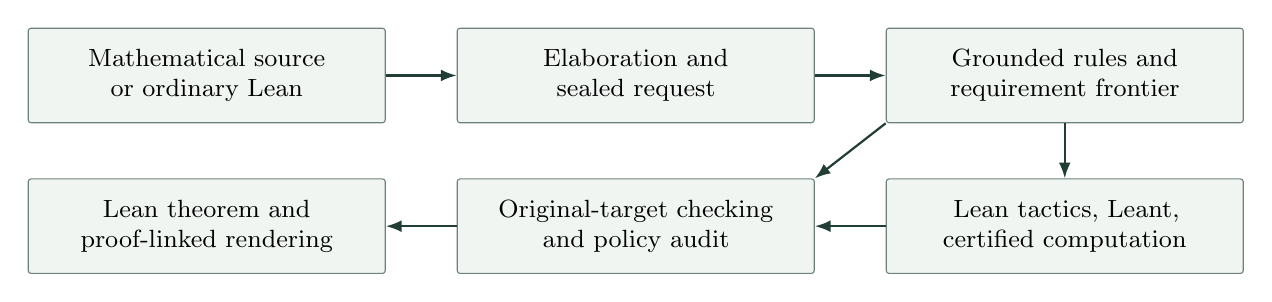
\begin{tikzpicture}[node distance=7mm and 9mm,
 box/.style={draw=ink!65,fill=soft,align=center,rounded corners=1pt,
 minimum height=12mm,text width=43mm,font=\small},
 arr/.style={-{Latex[length=2mm]},draw=ink,thick}]
\node[box] (src) {Mathematical source\\or ordinary Lean};
\node[box,right=of src] (req) {Elaboration and\\sealed request};
\node[box,right=of req] (front) {Grounded rules and\\requirement frontier};
\node[box,below=of front] (prov) {Lean tactics, Leant,\\certified computation};
\node[box,left=of prov] (check) {Original-target checking\\and policy audit};
\node[box,left=of check] (out) {Lean theorem and\\proof-linked rendering};
\draw[arr] (src)--(req);\draw[arr] (req)--(front);\draw[arr] (front)--(prov);
\draw[arr] (prov)--(check);\draw[arr] (check)--(out);
\draw[arr] (front.south west)--(check.north east);
\end{tikzpicture}
\end{center}
The upper and right-hand components may fail, search heuristically, or be
replaced. They never acquire authority to change the sealed request. The
renderer is an output view, not the source of the theorem's truth.

\subsection{The stopping rule is deliberately strict}
If an equally equipped Lean library and tactic interface performs as well as
the property-aware layer, keep the library, services, and renderer; do not
force a new language. If the property layer helps but the narrative surface
adds errors or repair cost, ship the property layer alone. If inference is
unpredictably expensive, require more explicit method choices rather than
hiding larger budgets behind a shorter source file.

\section{How to evaluate Fennel rather than its packaging}
\label{sec:evaluation}

\subsection{Matched experimental arms}
A useful experiment gives all comparable arms access to the same mathematical
knowledge and automation. The following design refines the controls in the
round-three reports \cite{synA,synB}.
\begin{center}\small
\begin{tabularx}{\textwidth}{@{}L{12mm}Y@{}}
\toprule
Arm & Available facilities\\
\midrule
$L_0$ & Ordinary Lean and existing automation.\\
$L_1$ & $L_0$ plus the new wrappers, property theorems, and registrations as explicit library interfaces.\\
$L_2$ & $L_1$ plus exactly the same synthesis and certificate services used by Fennel.\\
$L_3$ & $L_2$ plus property-implicit application, evidence indexing, and requirement-frontier diagnostics.\\
$L_4$ & $L_3$ plus the mathematical input surface.\\
$R$ & $L_2$ plus a read-only compact renderer, without property-aware input.\\
\bottomrule
\end{tabularx}
\end{center}
The key incremental contrasts are $L_3-L_2$, $L_4-L_3$, and $R-L_2$. Comparing
only $L_4$ with an under-equipped baseline would attribute library development
and stronger automation to syntax.

\subsection{Tasks and measurements}
Use mathematical statement preservation, authoring, and repair tasks.
The development suite includes the examples in this article; a separately
selected held-out suite should include new analysis, algebra, and relational
behavior cases. Preregister the selection and failure classification before
seeing which arm succeeds.

Measure completed correct tasks, active authoring time, explicit interventions,
incorrect accepted statements, misunderstood assumptions, repair effort after
controlled changes, and user confidence in the correct result. Measure
elaboration time, kernel-checking time, proof DAG and serialized proof size,
index size, registrations attempted, service calls, and frontier width
separately. Record cold and warm runs, toolchain pins, hardware, and budgets.
Shorter source is useful only in conjunction with these outcomes.

For a reading test, remove the implementation labels and ask readers to recover
the quantifiers, domain, equality kind, remaining premises, constructed
witnesses, and required method from the compact view. Include deliberately
nearby statements: a.e. versus everywhere, a Lipschitz bound versus the least
bound, and one witness versus a complete solution description. A reader who
mistakes any of these has detected a semantic failure of compression.

\subsection{A proposed acceptance suite}
\begin{longtable}{@{}L{.18\textwidth}L{.33\textwidth}L{.41\textwidth}@{}}
\toprule
Family & Positive fixture & Mutation and required response\\
\midrule\endhead
Derivative form & Finite product formula at every parameter. & Request quotient form at a zero factor: keep the exact target and expose or reject its guard.\\
Local induction & Equality on an open region with the point generalized. & Specialize the induction hypothesis too early: reject the locality route, not the theorem as false.\\
Exact quotient & The inhabited tuple $(3,2,5)$. & Use the four neighboring tuples: identify operation-specific failure; no full-package contradiction shortcut in the arithmetic method.\\
Tensor witness & Every factor finite/free, with naturality. & Drop factor finiteness: do not infer finite $W$ from finite indexing alone.\\
Almost everywhere & A correct integral congruence for the fixed measure. & Change the measure or use point evaluation: require the missing transport theorem.\\
Quantifier order & A fixed-countable-family a.e. transport under its theorem. & Aggregate the uncountable singleton family: do not move the quantifiers.\\
Source behavior & Affine length theorem over realized list inputs. & Supply an unrealizable positive length for \code{List Empty}: reject the proposed refutation.\\
Joint behavior & A paired observation from one input. & Combine individually realizable but incompatible observations: require joint realization.\\
Identity & Unchanged target and context with an accepted certificate. & Change a structure, universe, index, binder, or displayed edit: recheck, never relabel.\\
Method & A proof constructed from permitted rules. & Return another valid route: reject only the required-method claim.\\
Computation & A certificate with correct arity and original-target bridge. & Alter a coefficient, omit a generator, or change an atom: reject the certificate.\\
Frontier & An unseeded cycle remains unresolved. & Self-justify a guard or report timeout as false: reject the inference.\\
\bottomrule
\end{longtable}
These are planned full-system tests. Only the finite-graph analogues explicitly
listed in Section~\ref{sec:prototype} have been executed here. The positive
fixture and expected failure \emph{kind} are as important as the mutated input.

\section{Related work and the intended research contribution}
\label{sec:related}
Liquid Types combine inference and predicate abstraction to make selected
refinement properties automatic \cite{liquid}. Fennel shares the idea that
expressive predicates need a restricted inference mechanism; it differs in
using Lean proof objects for arbitrary mathematical propositions and in
exposing unresolved sufficient routes as an authoring interface. It does not
claim principal refinements in unrestricted dependent mathematics.

Dijkstra monads provide a disciplined relationship between effectful programs
and specification transformers \cite{dm}. They are an appropriate foundation
for effectful behavioral interfaces. Fennel's residual proof frontier is not
a general weakest-precondition calculus: it is a graph-relative account of
selected theorem routes, including mathematics unrelated to program execution.

ATMS labels are the direct precedent for the minimal-support data structure
\cite{atms}. Fennel's difference lies in proof-producing registration,
exact-statement preservation, absence of default truth assumptions, and its
proposed integration with a mathematical language. The antichain theorem is
presented as the relevant specialization with an explicit proof, not as a new
invention in inference algorithms.

Within the campaign, Trellis supplies finite qualifier closure; Schist supplies
backward sufficient-requirement reasoning; Karst and other proposals emphasize
scope and realizability; the two syntheses put these together into an
obligation-frontier interface \cite{trellis,synA,synB}. Fennel makes the
alternative-support semantics executable and states its limits, while leaving
most of the agreed core unchanged. Existing \code{fun_prop} and Lean's
verification-condition machinery further reduce the amount of new technology
that is justified \cite{funprop,mvcgen}.

The central untested research claim is therefore narrow: \emph{proof-carrying,
operation-specific residual requirements can improve mathematical authoring,
comprehension, and repair beyond a library and solver stack exposing the same
theorems explicitly}. The supplied experiment validates a small mechanism
needed by that claim, not the claim itself.

\section{Conclusion}
Fennel proposes a language in which a mathematical object keeps its identity,
its behavior has a precise contract, and an omitted justification remains a
typed, inspectable obligation. The surface is concise because it delegates
repeatable work to theorem-backed consumers, not because it makes assumptions
invisible. The automatic layer is predictable only within declared bounds;
when several sufficient routes are available, it carries their proofs and
supports rather than pretending that one chosen route is mathematically
necessary.

The most important design choice is not a keyword. It is the separation of
fixed statements, authorized constructions, proved properties, and outstanding
requirements. This separation lets a derivative retain its locality, an exact
quotient retain its divisibility, a behavior model retain its realization
conditions, and a CAS answer retain its actual guarantee.

The next useful artifact is a narrow Lean integration evaluated against an
equally equipped Lean baseline. A primitive kernel refinement remains a
possible later optimization, not a prerequisite. The successful outcome could
be a new language, a small elaborator extension, or simply a better mathematical
library and renderer. In all three cases the guiding principle is the same:
\emph{omit proof plumbing from the author's argument, but never omit it from
the system's account of why the argument is valid.}

\appendix
\section{Reproducing the companion experiment}
The package uses Python's standard library and does not download dependencies.
From the package root:
\begin{lstlisting}
python prototype/fennel.py prototype/quotients.fnl --out prototype/generated
python prototype/test_fennel.py
python prototype/stress_frontiers.py
\end{lstlisting}
The first command emits JSON certificates, ordinary conditional Lean source,
and an authoring-status summary. The second reruns the boundary tests and
finite reference comparison. The third reruns the exponential-output example.
Generated Lean files require a separate Lean compilation before any
kernel-validation claim is made. No toolchain-dependent Mathlib theorem names
are used in those opaque-proposition exports.

To build this article, run \code{pdflatex -interaction=nonstopmode -halt-on-error
Fennel.tex} three times, or use \code{latexmk -pdf Fennel.tex}. The bibliography
is embedded; no BibTeX run is necessary. The PDF was built and visually
inspected for this delivery.

\section{Evidence ledger}
\begin{center}\small
\begin{tabularx}{\textwidth}{@{}L{.32\textwidth}YY@{}}
\toprule
Item & Evidence status & Explicit limit\\
\midrule
Finite frontier theorem & Written proof in this article. & Fixed ground graph and independent proposition roots only.\\
Statement noninterference & Written proof of the specified transition invariant. & Not a theorem about an implemented Lean elaborator.\\
Primitive refinement conservativity & Written translation argument. & Only the explicit-evidence refinement fragment.\\
Python parser/planner/checker & Implemented and executed. & No arbitrary dependent types or Lean expression semantics.\\
Generated Lean & Produced from checked finite certificates. & Not compiled in this runtime.\\
Frey helper and round-three Lean cores & Historical checks reported in the requested syntheses. & Not rerun here; not measurements of Fennel.\\
Full mathematical syntax & Design examples. & Not accepted by the shipped finite parser.\\
CAS and Leant integration & Typed interface designs. & No end-to-end adapters executed here.\\
Authoring/comprehension benefit & Proposed evaluation. & No empirical gain established.\\
\bottomrule
\end{tabularx}
\end{center}

\section{Source pins and reading scope}
The immutable snapshots used for the repository review are:
\begin{center}\small
\begin{tabularx}{\textwidth}{@{}L{.31\textwidth}Y@{}}
\toprule
Repository & Commit\\
\midrule
Brainstorm & \code{bf3333905995060870f8585e297ffc16f3fe7e86}\\
ProveIt & \code{24ce8bd743eaab64a91ce90725ea00f498d319d2}\\
Fermat repository & \code{aa2d8b34692b16c70f699536de0d8e75b9a3e9ef}\\
Leant & \code{3a40904be8a410d832d9ab6900b3d3e7b425eccb}\\
\bottomrule
\end{tabularx}
\end{center}
The main synthesis sources were read closely, including their reconciliation
and fourth-round questions. Their included crosswalk and appendix files were
not separately exhaustively reviewed. Trellis's typing and finite-closure
sections were read directly. The four cited mathematical source files were
read in full; Leant's verification and Length-handoff modules were inspected
in the ranges recorded in the manifest. Public Lean documentation was accessed
on 6 September 2026 and may describe a newer toolchain than the prior syntheses'
Lean 4.32.0 experiments. Version-specific execution claims must therefore be
checked at the selected project pin, not inferred from a moving ``latest'' page.

\begin{thebibliography}{99}
\small
\setlength{\itemsep}{2pt}
\setlength{\parskip}{0pt}
\bibitem{synA} Brainstorm campaign.
\emph{From Properties to Proof Obligations: Round 3 Synthesis}.
6 September 2026. Main source at the Brainstorm pin listed above:
\href{https://github.com/VladimirReshetnikov/Brainstorm/blob/bf3333905995060870f8585e297ffc16f3fe7e86/docs/round-3/synthesis/unified-report.tex}{\nolinkurl{docs/round-3/synthesis/unified-report.tex}}.

\bibitem{synB} Brainstorm campaign.
\emph{Nine Refinements: Property-Aware Typing in a Mathematician's Proof Language over Lean}.
6 September 2026. Reconciled main source:
\href{https://github.com/VladimirReshetnikov/Brainstorm/blob/bf3333905995060870f8585e297ffc16f3fe7e86/docs/round-3/unified_report/unified_report.tex}{\nolinkurl{docs/round-3/unified_report/unified_report.tex}}.

\bibitem{trellis} Brainstorm campaign. \emph{Trellis}, round-three proposal.
Core typing and finite qualifier calculus, source lines 300--440:
\href{https://github.com/VladimirReshetnikov/Brainstorm/blob/bf3333905995060870f8585e297ffc16f3fe7e86/docs/round-3/ideas/trellis/trellis.tex#L300-L440}{\nolinkurl{docs/round-3/ideas/trellis/trellis.tex}}.

\bibitem{qpoch} Vladimir Reshetnikov and contributors. ProveIt.
\emph{Derivatives of finite q-Pochhammer symbols in the parameter}.
\href{https://github.com/VladimirReshetnikov/ProveIt/blob/24ce8bd743eaab64a91ce90725ea00f498d319d2/Analysis/FabiusFunction/Lean/FabiusFunction/QPochhammerDerivative.lean}{\nolinkurl{Analysis/FabiusFunction/Lean/FabiusFunction/QPochhammerDerivative.lean}}.
Declarations \code{hasDerivAt_finiteQPochhammerIn},
\code{hasDerivAt_finiteQPochhammerIn_of_ne_zero}, and
\code{hasDerivAt_finiteQPochhammerIn_comp}.

\bibitem{ode} Vladimir Reshetnikov and contributors. ProveIt.
\emph{Iterated derivatives of a solution of an autonomous equation}.
\href{https://github.com/VladimirReshetnikov/ProveIt/blob/24ce8bd743eaab64a91ce90725ea00f498d319d2/Analysis/FabiusFunction/Lean/FabiusFunction/AutonomousIteratedDeriv.lean}{\nolinkurl{Analysis/FabiusFunction/Lean/FabiusFunction/AutonomousIteratedDeriv.lean}}.
Declaration \code{AutonomousODE.iteratedDeriv_eq_comp}.

\bibitem{frey} Anthropic Fermat repository contributors.
\href{https://github.com/anthropics/fermats-last-theorem/blob/aa2d8b34692b16c70f699536de0d8e75b9a3e9ef/P2M/Sol/S_FreyPackage_freyCurveInt_map.lean}{\nolinkurl{P2M/Sol/S_FreyPackage_freyCurveInt_map.lean}}.
In particular, \code{FreyArith.freyCurveInt_map} and its coefficient divisibility proofs.

\bibitem{tensor} Anthropic Fermat repository contributors.
\href{https://github.com/anthropics/fermats-last-theorem/blob/aa2d8b34692b16c70f699536de0d8e75b9a3e9ef/P2M/Sol/S_Algebra_exists_algHom_equiv_pi.lean}{\nolinkurl{P2M/Sol/S_Algebra_exists_algHom_equiv_pi.lean}}.
The \code{solution} declaration explicitly assumes finite and free factors
and concludes with a natural representation equivalence.

\bibitem{leantV} Vladimir Reshetnikov and contributors. Leant.
\href{https://github.com/VladimirReshetnikov/Leant/blob/3a40904be8a410d832d9ab6900b3d3e7b425eccb/src/Leant/Synth/Verification.hs#L1-L180}{\nolinkurl{src/Leant/Synth/Verification.hs}}, lines 1--180.

\bibitem{leantH} Vladimir Reshetnikov and contributors. Leant.
\href{https://github.com/VladimirReshetnikov/Leant/blob/3a40904be8a410d832d9ab6900b3d3e7b425eccb/src/Leant/Synth/Length/Handoff.hs#L1-L180}{\nolinkurl{src/Leant/Synth/Length/Handoff.hs}}, lines 1--180.

\bibitem{leanTypes} Lean developers. \emph{The Lean Language Reference: The Type System}.
\href{https://lean-lang.org/doc/reference/latest/The-Type-System/}{Official reference}, accessed 6 September 2026.

\bibitem{leanTactics} Lean developers. \emph{The Lean Language Reference: Tactic Reference}.
\href{https://lean-lang.org/doc/reference/latest/Tactic-Proofs/Tactic-Reference/}{Official reference}, accessed 6 September 2026.

\bibitem{leanAxioms} Lean developers. \emph{The Lean Language Reference: Axioms}.
Sections on parametricity, native execution assumptions, and displaying axiom dependencies.
\href{https://lean-lang.org/doc/reference/latest/Axioms/}{Official reference}, accessed 6 September 2026.

\bibitem{funprop} Mathlib contributors. \emph{Mathlib.Tactic.FunProp}.
\href{https://leanprover-community.github.io/mathlib4_docs/Mathlib/Tactic/FunProp.html}{Official generated documentation}, accessed 6 September 2026.

\bibitem{mvcgen} Lean developers. \emph{The Lean Language Reference: The mvcgen Tactic}.
\href{https://lean-lang.org/doc/reference/latest/The--mvcgen--tactic/}{Official reference}, accessed 6 September 2026.

\bibitem{atms} Johan de Kleer. Problem Solving with the ATMS.
\emph{Artificial Intelligence} 28 (1986), 197--224.
\href{https://dekleer.org/Publications/Problem\%20Solving\%20with\%20the\%20ATMS.pdf}{Author-hosted paper}, especially pp.\ 197--201 on supporting environments and interface correctness.

\bibitem{liquid} Patrick M. Rondon, Ming W. Kawaguchi, and Ranjit Jhala.
Liquid Types. \emph{Proceedings of PLDI}, 2008.
\href{https://goto.ucsd.edu/~rjhala/papers/liquid_types.html}{Authors' publication page}.
DOI: 10.1145/1375581.1375602.

\bibitem{dm} Danel Ahman, C\u{a}t\u{a}lin Hri\c{t}cu, Kenji Maillard,
Guido Mart\'{i}nez, Gordon Plotkin, Jonathan Protzenko, Aseem Rastogi, and Nikhil Swamy.
Dijkstra Monads for Free. \emph{Proceedings of POPL}, 2017.
\href{https://fstar-lang.org/papers/dm4free/}{Project publication page}.
DOI: 10.1145/3009837.3009878; arXiv:1608.06499.
\end{thebibliography}
\end{document}
